%% PARCFD PAPER FOR JOURNAL SUBMISSION:
% TARGETS IN ORDER
% https://www.journals.elsevier.com/computer-physics-communications
% https://www.journals.elsevier.com/future-generation-computer-systems
% https://www.journals.elsevier.com/computers-and-fluids

% That's a fine journal and all. Very similar metrics to JCP.
% BUT Computer Physics Communications is really right up the alley here since I've made what could be considered a framework and it has much better metrics than the other two.  And their acceptance rate was 41% last year.

%% Paper on novel parallel decomposition method for accelerating 1D simulations on GPU architecture.
\pdfoutput=1
\pdfminorversion=5 % necessary for EES
%
\documentclass[12pt,number,sort&compress,preprint]{elsarticle}

% better printing of numbers
\usepackage[utf8]{inputenc}
\usepackage[T1]{fontenc}
\usepackage[english]{babel}
\usepackage{textcomp}
\usepackage{booktabs,multicol}

\usepackage[hyphens]{url}
\biboptions{sort&compress, square, comma}
\usepackage[breaklinks=true, linkcolor=blue, citecolor=blue, colorlinks=true]{hyperref}

\usepackage{latexsym, amsmath, amssymb}
\usepackage{graphicx, color, xcolor, wrapfig, subcaption}
\usepackage{listings}

\usepackage{nicefrac}

\usepackage[binary-units]{siunitx}

%%%%%%%%%%%%%%%%%%%%%%%%%%%%%%%%%%
% ADDING LINENUMBERS FOR REVIEWING:
\usepackage{lineno}

\sisetup{group-separator={,},
	detect-all,
	binary-units,
	list-units = single,
	range-units = single,
	range-phrase = --,
	per-mode = symbol-or-fraction,
	separate-uncertainty = true,
	multi-part-units = single,
	list-final-separator = {, and }
%    scientific-notation = fixed
}

\newcommand{ \ddt } [1] { \frac{ \partial #1 }{ \partial t } }
\newcommand{ \ddx } [1] { \frac{ \partial }{ \partial #1 } }
\newcommand{ \dydx } [2] { \frac{ \partial #1 }{ \partial #2 } }
\newcommand{ \ddydxx } [2] { \frac{ \partial^2 #1 }{ \partial #2^2 } }
\newcommand{ \us } [0] {\textunderscore}

\definecolor{dkgreen}{rgb}{0,0.6,0}
\definecolor{gray}{rgb}{0.5,0.5,0.5}
\definecolor{mauve}{rgb}{0.58,0,0.82}

\lstset{ %
  language=C,
  breaklines=true,
  columns=flexible,
  basicstyle=\tiny \ttfamily,
  backgroundcolor=\color{white},
  showspaces=false,
  showstringspaces=false,
  showtabs=false,
  frame=single,
  tabsize=2,
  captionpos=b,
  keywordstyle=\color{blue},
  commentstyle=\color{dkgreen},
}

% C++ macro
\def\CC{{C\nolinebreak[4]\hspace{-.05em}\raisebox{.4ex}{\footnotesize ++}}}


%disable
\usepackage[textsize=footnotesize]{todonotes}
\setlength{\marginparwidth}{2cm}

\graphicspath{ {images/} }

% Define commands to assure consistent treatment throughout document
\newcommand{\eqnref}[1]{(\ref{#1})}
\newcommand{\class}[1]{\texttt{#1}}
\newcommand{\package}[1]{\texttt{#1}}
\newcommand{\file}[1]{\texttt{#1}}
\newcommand{\BibTeX}{\textsc{Bib}\TeX}

%\newcommand{\TheAuthors}{Daniel J.~Magee and Kyle E.~Niemeyer}
%\headers{GPU-based swept time-space decomposition}{\TheAuthors}


\usepackage[normalem]{ulem}

\newcommand{\hfigs}[5]{
    \begin{figure}[!tb]
        \centering
        \begin{subfigure}[t]{.48\textwidth}
            \centering
            \includegraphics[width=\textwidth]{#1}
            \caption{#3}
            \label{f:#1}
        \end{subfigure}
        \hfill
        \begin{subfigure}[t]{.48\textwidth}
            \centering
            \includegraphics[width=\textwidth]{#2}
            \caption{#4}
            \label{f:#2}
        \end{subfigure}
        \caption{#5}
        \label{f:#1Result}
    \end{figure}
}

\def\WCPU{Intel Xeon 2630-E5 v3}
\def\WGPU{Nvidia Tesla K40c}
\def\CCPU{Intel Xeon 2660-E5 v3}
\def\CGPU{Nvidia Tesla K40m}

\newcommand{\tx}[1]{$#1\times$}

\begin{document}

\begin{frontmatter}

\title{Applying the swept rule for explicit PDE solutions on heterogeneous computing systems}

\author[OSU]{Daniel J.~Magee}
\author[OSU]{Kyle E.~Niemeyer\corref{cor1}}
\ead{kyle.niemeyer@oregonstate.edu}

\cortext[cor1]{Corresponding author}
\address[OSU]{School of Mechanical, Industrial, and Manufacturing Engineering,
Oregon State University, Corvallis, OR, USA
}

% We present recent work on the swept rule, a domain decomposition strategy for explicit solutions to partial differential equations, on heterogeneous, distributed architectures, in particular those commonly found on compute clusters containing GPGPU accelerators.
\begin{abstract}
    
Applications that exploit the architecural details of high performance computing (HPC) systems have become increasingly invaluable in academia and industry over the past two decades.
The most important hardware development of the last decade in HPC has been the General Purpose Graphics Processing Unit (GPGPU), a class of massively parallel devices that now contributes a substantial balance of the computational power in the top 500 supercomputers.
As these systems grow small costs such as latency, the fixed cost of memory accesses, accumulate over the numerous iterations in a large simulation becoming a significant barrier to performance. 
The swept time-space decomposition rule is a communication-avoiding technique for time-stepping stencil update formulas that attempts to sidestep a portion of the latency costs.
This work extends the swept rule by targeting heterogeneous, CPU\slash GPU architectures representative of current and future HPC systems.
We compare our approach to a naive decomposition scheme with two test equations using an MPI+CUDA pattern on 40 processes over two nodes containing one GPU.
We show that the swept rule produces a \SIrange{4}{18}{$\times$} speedup with the heat equation and a \SIrange{1.5}{3}{$\times$} speedup on the Euler equations using the same processors and work distribution.
These results demonstrate the effectiveness of the swept rule for different equations and numerical schemes on compute systems that incur substantial latency costs.

\end{abstract}

\begin{keyword}
    Domain decomposition \sep Heterogeneous computing \sep partial differential equations \sep computational fluid dynamics \sep communication-avoiding algorithms
\end{keyword}

\end{frontmatter}

% FOR REVIEWING
\linenumbers

\section{Introduction}

Computational fluid dynamics (CFD) simulations are at the heart of technological development in industries vital to high and rising standards of living around the world.
Performing simulations at the level of fidelity necessary for continual insight consumes more resources than individual workstations can reasonably accommodate.
As a result these simulations are generally performed on high performance computing (HPC) systems with many nodes each containing several multi-core CPUs---and increasingly with other specialized ``accelerator'' co-processors.
These heterogeneous, that is containing more than one computational architecture, computing systems have become ubiquitous in areas of research dependent on large amounts of data, complex numerical transformations, or densely connected systems of constraints.
Addressing these problems reveals a further horizon where new, more complex questions emerge.
Steady progress requires increasing development in large-scale computational systems; solutions from hardware and software are required to supply the necessary throughput for demand in numerous fields, including several not known for their reliance on computational science such as medical diagnostics, genetics, marketing and biology.

In many ways recent improvements in computational capacity has been sustained through the development of accelerators or co-processors, such as general purpose graphics processing units (GPGPUs), which augment the computational capabilities of the CPU.
These devices have grown in power and complexity over the last decade, leading to an increasing reliance on them for enabling efficient floating-point computation on HPC systems~\cite{ALEXANDROV20161}.
However, as these systems grow in complexity, computational power, and physical size, latency and bandwidth costs limit the performance of applications that require regular inter-node communication.
Bandwidth is the amount of memory that can be communicated per unit of time, and latency is the fixed cost of a communication event---the travel time of the leading bit in a message.
Solving partial differential equations (PDEs) on HPC systems using explicit numerical methods involves domain decomposition (a heuristic for dividing the computational domain across the processors), with required inter-node communication of small data packets for boundary information at every time step.
The frequency of these communication events renders their fixed cost, latency, a significant barrier to the performance of these simulations.

This work is aligned with the overall goals of the HPC development community and seeks to address, however nascently, two of the challenges on the route to exascale computing systems identified by Alexandrov in his editorial in a recent special issue of the \textit{Journal of Computational Science}: the need for ``novel mathematical methods\dots{} to hide network and memory latency, have very high computation\slash communication overlap, have minimal communication, have fewer synchronization points'', and ``mathematical methods developed and corresponding scientific algorithms need to match these architectures [standard processors and GPGPUs] to extract the most performance. This includes different system-specific levels of parallelism as well as co-scheduling of computation''~\cite{ALEXANDROV20161}.

In this paper we describe the development and performance analysis of a PDE solver targeting heterogeneous computing systems (i.e., CPU\slash GPU) using the swept rule, a communication-avoiding, latency-hiding domain decomposition scheme~\cite{alhubail:16jcp,Alhubail:2016arxiv}.
Section~\ref{sec:hRwork} describes recent work on domain decomposition schemes with particular attention to applications involving PDEs and heterogeneous systems.
Section~\ref{sec:obj1} describes the questions this study seeks to answer.
Section~\ref{sec:hMethods} introduces swept time-space decomposition and discusses the experimental hardware, procedure, and factors used to evaluate the program performance.
This section also analyzes and justifies our design decisions concerning constant elements of the program that could have potentially been investigated.
In Section~\ref{sec:hResults} we present the results of the tests and describe the hardware and the testing procedures used; lastly in Section~\ref{sec:hConc} we draw further conclusions, describe future challenges, and outline plans for prioritizing and overcoming them.



\section{Related Work} \label{sec:hRwork}

In our previous work~\cite{OurJCP} we investigated methods for exploiting the memory hierarchy on a single GPU in a swept time-space solver for stencil computations. 
Alhubail et al.~\cite{MaithamRepo, alhubail:16jcp, Alhubail:2016arxiv} first developed the swept rule for CPU-based operation in one and two dimensions; Wang also demonstrated how complex numerical schemes can be decomposed into ``atomic'' update formulas, a series of steps requiring only a three-point stencil, suitable for the swept rule~\cite{WangDecomp}.
We use this technique, which we refer to as ``\texttt{lengthening}'', in the implementation of the swept rule discussed in this work
and contrast it with another method for dealing with complex schemes, ``\texttt{flattening}'', which we used in our previous GPU-only used~\cite{OurJCP}.
Section~\ref{sec:hPrimaryData} quantitatively compares the two techniques. 
In addition, Alhubail and Wang applied this procedure to automatically generate C source code for solving the heat and Kuramoto--Sivashinsky equations using the swept rule on CPU-based systems~\cite{AIAAWang}.
These articles comprise the body of work on the swept rule to date, which this paper expands upon.

Memory hierarchies are defined by a series of locations where memory is scarce and fast to plentiful and slow.
By working on data in the limited fast memory space as long as possible, communication-avoiding algorithms accelerate computation by reducing inter-process communication or global memory access cost in parallel programs.
Swept time-space decomposition is a type communication-avoiding algorithm because it seeks to reduce the number of communication events between the processor and less accessible memory resources.
Unlike most communication-avoiding algorithms though, it does not perform redundant operations.
The heterogeneous communication-avoiding LU factorization algorithm presented by Baboulin et al.~\cite{BABOULIN201217} investigates the task splitting between the GPU and CPU and minimizes inter-device communication.
Their results show an appreciable benefit from splitting the types of tasks performed on the CPU and GPU, which reduces overall communication and effectively overlaps computation and communication.

Studies of stencil optimization techniques over the last decade often address concerns closely related to the work presented here.
Datta et al.~\cite{VolkovDatta2008} explored domain decomposition with various launch parameters on heterogeneous architectures and nested domain decomposition within levels of the memory hierarchy.
Malas et al.~\cite{MalasHager} previously explored similar diamond tiling methods by using the data dependency of the grid to improve cache usage.

Swept time-space decomposition is also conceptually related to parallel-in-time methods~\cite{Gander2015}, such as multigrid-reduction-in-time~\cite{falgout2014parallel}.
These algorithms overcome the interdependence of solutions in the time domain in order to parallelize it as if it were spatial.
This technique iterates over a series of fine and coarse grids using an initial guess for the entire solution domain and effectively smoothes out the errors in the solution.
Historically, parallel-in-time methods were considered unsuitable for nonlinear problems since the use of coarse grids substantially degraded efficiency and accuracy~\cite{alhubail:16jcp}.
However, recent developments applying optimization and auto-tuning techniques have matched the scaling of linear solvers~\cite{MGRITImprove}.
Parareal is a parallel-in-time method that solves multiple time steps in parallel on a fine grid
and corrects the results on a coarse grid until the solution converges, resulting in a solution with the accuracy of the fine grid.
Wu and Zhou proposed a new local time-integrator for this method that shows considerable promise
for accelerating convergence rates in fractional differential equations~\cite{PararealWu}.

As these distributed, remote, multi-node systems and have become increasingly heterogeneous in recent years, implementing CFD codes effecively on these systems grown more complex.
Therefore, domain decomposition on these systems has received a good deal of recent attention.
In particular, Huerta et al. used methods from process engineering, including experimental design and non-continuous linear models in an experimental parameter space paradigm, to investigate the performance of a well known benchmark used to rank HPC clusters, HPL, with respect to workload division on a heterogeneous system~\cite{DOEbenchmarks}.
This technique shows considerable promise and could be considered for future studies of the swept rule with a more mature code base.
However, at our current stage, such a thoroughgoing analysis would not provide actionable insights beyond what we have already gleaned from our comparatively simpler methods.


\section{Objectives} \label{sec:obj1}

This study concerns the construction and analysis of a program that applies swept time-space decomposition to explicit stencil computations intended for distributed memory systems with heterogeneous architecture, that is, computational operations are performed by several CPUs and co-processors, in particular Nvidia GPUs.
The software is written in \CC{} and CUDA and uses the Message Passing Interface (MPI) library~\cite{Clarke1994} to communicate between CPU processes and the CUDA API to communicate between the GPU and the CPU.

While stencil computation is a relatively simple procedure, applying linear operations to individual spatial
points and their neighbors and the complexities introduced both by a heterogeneous architecture and swept
time-space decomposition require a significant number of design decisions.
In this work we investigated the performance impact of the most immediately salient and configurable decisions,
and constrained other potential variations with reasonable or previously investigated values.
Our investigations focus on answering the following questions:
\begin{enumerate}
    \item Does the swept rule reduce time-cost under optimal launch bounds over the domain of grid sizes?
    \item How much work should we give to the GPU in a heterogeneous system?
    \item How should we decompose the stencils in multi-step methods? (Further discussion in Section~\ref{sec:hPrimaryData})
    \item Does the size of the domain of dependence substantially affect performance?
\end{enumerate}



\section{Methodology} \label{sec:hMethods}

\input{Methodology/Sweptdecomposition.tex}


\subsection{Experimental method} \label{sec:ExpMethod}

We endeavor to address the questions presented in Section~\ref{sec:obj1} by varying
three primary attributes of the decomposition: threads per block, GPU affinity, and grid size.
We repeatedly executed our two test equations, the heat and Euler equations, over the
experimental domain of these variables using \texttt{Swept} and \texttt{Classic}, exchanging borders every
sub-time step, decomposition methods.
In our program implementing the swept rule in one-dimension on heterogeneous systems, hSweep,
threads per block is synonymous with the size of the domain-of-dependence, but we refer to it using GPU terminology because each domain is launched as a block of threads on the GPU.
A block is an abstract grouping of threads that share an execution setting, a streaming multiprocessor, and access to a shared memory space, a portion of the GPU L1 cache.
hSweep uses the swept rule to avoid communication between devices and processes and exploits the
GPU memory hierarchy to operate on shared memory quantities closer to the processor.
Since this multi-level memory scheme influences the swept-rule performance and GPU execution, the resultant effects are difficult to predict.
The independent variables GPU affinity and grid size are more straightforward.
The grid size is the total number of spatial points in the simulation domain, and is provided
by the user; however, the program revises this number to provide a grid that fits the other program settings
that the grid must accommodate: the threads per block, GPU affinity, and number of processes.
The GPU affinity is the portion of the computational grid that is processed by the GPU,
expressed as a ratio of the number of domains-of-dependence assigned to the GPU to those assigned to a single MPI process (on a CPU core).
GPU affinity, like the other experimental variables, should be given as an integer, since we have
determined that it is beneficial for the GPU to handle a larger portion of the overall grid
than a single MPI process.

In our previous study of the swept rule~\cite{OurJCP}, the experimental domain was clearly
defined by the particular properties of GPU architecture.
Because a warp contains 32 threads and a block cannot exceed 1024 threads, here we constrained
the number of threads per block, which is also the width of the domain of dependence, in our experiments
to be a power of 2 from \numrange{32}{1024}.
To enforce regularity, we constrained our experimental problem size---the number of spatial points in the
grid---to be a power of 2 larger between \num{1024} and $2^{21}$.

Using CPU parallelism across 40 processes and GPU affinity as a variable of interest in this study, eliminates the potential for regularity in the experimental grid.
To remedy this, we relaxed the constraints on the experimental launch conditions so that the number of
threads per block is required to be a multiple of 32 from \numrange{32}{1024} rather than a power of two.
In addition, at runtime the program uses the number of processes, threads per block, GPU affinity,
and desired grid size to determine the closest grid size to the requested value that accommodates the constraints.
This results in different grid sizes for the same experimental settings.
To assess the performance at various settings, we interpolated each result to the requested grid size
from the actual grid size.

The addition of GPU affinity as an independent variable introduces further complication to the experimental domain.
While our experiments are constrained by GPU architecture in threads per block and by the number
of processes and blocks in problem size, we initially have no clear indication of what the
experimental limits of GPU affinity should be---so we took an iterative approach.
First, we ran a screening study and executed the programs over a broad range of conditions:
eight block sizes from \numrange{64}{768}, 11 GPU affinities from \numrange{0}{80}, and
four grid sizes from \numrange{5e5}{e7}.
This showed us that the best affinity for all the programs would likely fall between \numrange{20}{60}
and that all threads per block values could provide the best performance.
This was somewhat disappointing, since we had hoped to narrow the range for both GPU affinity and
threads per block further in order to experiment on a finer increment of grid size in a reasonable amount of time.
For the final experiment, we used the same block sizes, GPU affinity values from \numrange{20}{60}
in increments of 4, and seven grid sizes over the same range.

In this study, we solve the one-dimensional heat equation using a first-order forward in time, central in space
method and Euler equations for a shock wave using a second-order finite-volume scheme with minmod limiter.
Explanations of these methods can be found in the appendix of our previous paper~\cite{OurJCP}.



\section{Results} \label{sec:hResults}

\subsection{Primary data structure} \label{sec:hPrimaryData}

Implementing the swept rule for problems amenable to single-step PDE schemes is straightforward,
but dealing with more realistic problems often requires more complex, multi-step numerical schemes.
Managing the working array and developing a common interface for these schemes, provokes design decisions that have substantial impacts on performance.

One strategy for dealing with this complexity we term \texttt{flattening} since it flattens the domain of dependence in the time dimension by using wider stencils and fewer sub-timesteps. 
This strategy is more memory efficient for the working array which contains instances of the primary data structure at each spatial point, but it cannot easily accommodate different methods and equations.
It also introduces additional complexity from parsing the arrays and requires additional register memory for function and kernel arguments and ancillary variables.

In the new implementation shown here we use the \texttt{lengthening} strategy, also referred to as ``atomic decomposition'', which is instantiated as a struct to generalize the stages into a user-defined data type~\cite{WangDecomp}.
It requires more memory to be used in the primary data structure; for instance, our \texttt{flattening} version of the Euler equations carried six doubles per spatial point since the pressure ratio used by the limiter was rolled into the flattened step.
These strategies are described in Figures~\ref{f:Longpseudo} and ~\ref{f:flatPseudo}. 
By restricting the stencil to three points, the \texttt{lengthening} method requires the pressure ratio to be stored and passed through the memory hierarchy meaning the data structure carries seven doubles per spatial point for the Euler equation.

\begin{figure}[bt]
    \begin{minipage}[t]{0.48\textwidth}
        \begin{lstlisting}
        // Q = {rho, rho*u, rho*E}
        struct states {
            double3 Q[2]; // State Variables
            double Pr; // Pressure ratio
        };

        __device__ __host__
        void stepUpdate(states *state, const int idx, const int tstep)
        {
            int ts = tstep % 4; // 4 is number of steps in cycle
            if (tstep & 1)  pressureRatio(state, idx, ts);
            else            eulerStep(state, idx, ts);
        }

        __global__ void classicStep(states *state, const int tstep)
        {
            int gid = blockDim.x * blockIdx.x + threadIdx.x + 1;
            stepUpdate(state, gid, tstep);
        }
        \end{lstlisting}
        \caption{Skeleton for the \texttt{lengthening} method in the \texttt{Classic} program. The \texttt{states} structure contains all the information to step forward at any point.  The user is only responsible for writing the \texttt{eulerStep} and \texttt{pressureRatio} functions and accessing the correct members based on the timestep count}
        \label{f:Longpseudo}
    \end{minipage}
    ~
    \begin{minipage}[t]{0.48\textwidth}
        \begin{lstlisting}
        __global__ void classicStep(const double *s_in, double *s_out, bool final)
        {
        int gid = blockDim.x * blockIdx.x + threadIdx.x;
        //number of spatial points - 1
        int lastidx = ((blockDim.x*gridDim.x));
        int gids[5];

        for (int k = -2; k<3; k++) gids[k+2] = (gid + k) % lastidx;

        //Final is false for predictor step, true otherwise.
        if (final) s_out[gid] += finalStep(s_in, gids);
        else       s_out[gid]  = predictorStep(s_in, gids);
        }
        \end{lstlisting}
        \caption{Skeleton for the \texttt{flattening} method in the \texttt{Classic} program. The sub-timesteps are compressed to a step with a wider stencil. The two arrays which alternate reading and writing are explicitly passed and traded in the calling function.}
        \label{f:flatPseudo}
    \end{minipage}
\end{figure}

To gauge the influence of this change in primary data structure, we implemented each combination of the classic and swept decomposition techniques using the \texttt{flattening} and \texttt{lengthening} data structures.
We applied these solvers to the Euler equations using the discretization and conditions described in Section~\ref{sec:ExpMethod}.
These programs use a single GPU as the sole computational device as opposed to the other results in this paper, which are evaluated with CPUs and GPUs on a heterogeneous platform.  

\hfigs{SpeedupAtomicArrayEuler}
{SpeedupAlgoAtomicArrayEuler}
{Speedup of \texttt{flattening} compared to the same scheme using \texttt{lengthening}.}
{Speedup of \texttt{Swept} program compared to \texttt{Classic} using each data structure strategy.}
{Performance comparison of the \texttt{flattening} and \texttt{lengthening} strategies solving the Euler equations on a single GPU.}

% \begin{figure}[htbp]
%     \centering
%     \includegraphics[width=.7\textwidth]{SpeedupAtomicArray}
%     \caption{Speedup of \texttt{flattening} compared to the same scheme using \texttt{lengthening} applied to the KS equation on the GPU only.}
%     \label{f:lflat}
% \end{figure}

Figure~\ref{f:SpeedupAtomicArrayEulerResult} compares the performance of the memory storage techniques in an
experiment executed on a workstation with an \WCPU{} and an \WGPU{}.
Figure~\ref{f:SpeedupAtomicArrayEuler} shows the speedup, the ratio of the average time per timestep, of a \texttt{lengthening} implementation compared to a \texttt{flattening} implementation for each domain decomposition scheme.
Figure~\ref{f:SpeedupAlgoAtomicArrayEuler} describes the effect that the choice of primary data structure has on the main quantity of interest in this project: the speedup of a \texttt{Swept} compared to a \texttt{Classic} program.

Figure~\ref{f:SpeedupAtomicArrayEuler} shows that the \texttt{flattening} strategy is faster than \texttt{lengthening} for both decomposition methods, and the speedup grows as the number of spatial points increases, but this performance difference and trend is more pronounced in a \texttt{Classic} program than a \texttt{Swept} one.
Much of the reason that \texttt{lengthening} is less performative for both decomposition methods--the performance sensitivity to irregularity in memory access patterns amplified by the array of sturctures used in \texttt{lengthening}--is particular to GPU architecture,  so it is difficult to generalize the results in this section to heterogeneous systems. 
The extra memory requirements of the \texttt{lengthening} method also consume limited shared memory resources on the GPU, which diminishes occupancy, the number of threads active on the GPU at any given time, in the \texttt{Swept} program and the L1 cache capacity used to accelerate global memory accesses on Kepler-generation GPUs in the \texttt{Classic} program.
While locality is a significant issue for effective CPU memory accesses, it has a larger impact on GPU performance.

These issues explain the general benefit of the \texttt{flattening} strategy, but they do not explain why these benefits are more pronounced in the \texttt{Classic} program.
First, the \texttt{lengthening} strategy, which requires more sub-timesteps per timestep in order to limit the stencil to three points, does not affect the number of kernels launches in the \texttt{Swept} program, but may increase the occurrence of these events in the \texttt{Classic} program.
In the case of the Euler equations, there are four sub-timesteps per timestep in our scheme using \texttt{lengthening} which is reduced to two with the \texttt{flattening} strategy; this causes the \texttt{Classic lengthening} program to launch twice as many kernels as it would with \texttt{flattening}. 
Also, the aforementioned structure of arrays paradigm used in the \texttt{lengthening} strategy increases the stride for memory accesses which has little effect on the \texttt{Swept} program since it uses mostly shared memory and this access pattern does not produce bank conflicts, but it does prevent global memory accesses from coalescing which is a significant portion of the \texttt{Classic} program cost.

Figure~\ref{f:SpeedupAlgoAtomicArrayEuler} shows what we found in our previous study of the Euler equations using the \texttt{flattening} method~\cite{OurJCP}.
It also shows that if we had used the \texttt{lengthening} strategy, we would have found that the swept decomposition scheme does provide a benefit compared to classic.
In any experimental algorithm, especially those involving emerging, parallel computational platforms, performance is dependent to various degrees on a multitude of implmentation details, and we feel that it is important to present these findings so that others who implement the swept rule will have a more thorough understanding of the tradeoffs inherent in particular program design choices.
In this case we have subjectively determined that the benefits the \texttt{lengthening} method provides: extensibility and regularity are of greater value than the absolute best performance.


\subsection{Swept Decomposition}  \label{sec:SweptDecompRslt}

All programs were compiled with the CUDA compiler \texttt{nvcc v8} and launched with \texttt{mpirun v3.1.4}.
Our study collects the average time per timestep over \num{4000} timesteps; 
The timing measurements include the onetime costs of device memory allocation and initial and final host-device memory transfers, this does not include the time cost of host-side memory management, grid generation, file I/O and initial condition calculations.
The heterogeneous swept rule algorithms and test cases were implemented in \texttt{hSweep v2.0}~\cite{hSweepz}.

\hfigs{BestRuntimeHeat}
{BestSpeedupHeat}
{Time cost of heat equation program at best launch condition.}
{Speedup of swept version at best launch condition.}
{Performance comparison of the hSweep heat equation programs.}

\hfigs{BestRuntimeEuler}
{BestSpeedupEuler}
{Time cost of Euler equation program at best launch condition.}
{Speedup of swept version at best launch condition.}
{Performance comparison of the hSweep Euler equations programs.}

We performed the tests on the \texttt{Classic} and \texttt{Swept}
programs on two nodes of the Oregon State University College of Engineering cluster.
Each node contains two sockets with~\CCPU{} processors with ten cores each operating at~\SI{2.60}{\giga\hertz}.
An~\CGPU{} GPGPU is available to one of these nodes through a PCI connection.

Figure~\ref{f:BestRuntimeHeat} compares the computational time cost per timestep of the heat equation programs
using the \texttt{Classic} and \texttt{Swept} algorithms.
These results are generally consistent with our expectations for several reasons.
First, we have observed that in previous studies~\cite{OurJCP, alhubail:16jcp}, that
\texttt{Swept} programs applied to simpler problems are highly performative when the processes operate but reach that
capacity at smaller grid sizes than \texttt{Classic} programs.
This difference in the capacity for increasing grid sizes narrows the performance advantage of \texttt{Swept} swiftly, and, since both algorithms scale similarly with grid size, the relative speedup of \texttt{Swept} declines as well although the absolute speedup remains constant.

Second, although the minimum grid size in this study is about \tx{100} larger
than our previous study, and the maximum grid size is about \tx{10} larger,
Figure~\ref{f:BestSpeedupHeat} shows a similar trend in the speedup of swept decomposition.
In general the speedup exhibited by the heterogeneous case is \tx{2} the speedup at the analogous grid size in the GPU-only case over the experimental range.
This relative speedup of the heterogeneous swept rule is expected since latency is a much larger cost in internode communication than within the GPU memory hierarchy or between the CPU and GPU. 

Figure~\ref{f:BestRuntimeEulerResult} compares the time cost per timestep of the \texttt{Classic} and \texttt{Swept} algorithms with the Euler equations and shows the same performance trends as the heat equation.
In this case, the communication costs that the program avoids are significant enough that swept decomposition provides a tangible benefit despite the extra complexity, management, and memory resources that it requires.
This shows that swept time-space domain decomposition is a viable method for complex equations in one dimension on systems with substantial communication costs and various architectures.

Figures~\ref{f:EulerContours} and~\ref{f:HeatContours} show contour maps of the results
of the complete experiment, as described at the end of Section~\ref{sec:ExpMethod}.
By creating similar maps in the first stage of the experiment, we were able to narrow the range of experimental variables to capture the best performance for each problem, algorithm, and grid size.
Figure~\ref{f:EulerContours} shows interesting characteristics of the programs that vary by runtime configuration and decomposition method.
Notably, these results show that for the Euler equations, the \texttt{Swept} program often achieves best performance at GPU affinities between \numrange{45}{55} and often does best with \num{768} grid points in the domain of dependence, but performs particularly poorly with \num{512} points.
From other perspectives the performance profile of the \texttt{Swept} Euler equations program appears quite regular, so a sudden drop in performance followed by a substantial increase is unexpected.
The consistency of the influence of GPU affinity allows further studies to explore more granular performance characteristics.
While the saddle along the threads per block axis is problematic for our
general recommendations, we also observe that the program consistently exhibits similar performance from~\numrange{192}{384} threads per block.

Additionally, we observe from these maps that \texttt{Swept} produces a more orderly performance profile than \texttt{Classic}.
For grids with less than \num{e6} spatial points, the classic decomposition technique produce peaks and valleys over a wide range of block sizes sizes and GPU affinities.
On larger grids, that disorder regularizes and the best performance occurs with smaller blocks and larger GPU affinities.
This suggests that we may have truncated the GPU affinity dimension prematurely in our experiments.
The regularity we observe in the experimental grid for \texttt{Swept} programs also extends in the grid size dimension as described by Figures~\ref{f:BestRuntimeHeatResult} and \ref{f:BestRuntimeEulerResult} show swept decomposition produces a nearly perfect power law curve for each problem quantified in Table~\ref{tab:tablefit}.

\begin{figure}[htbp]
    \centering
    \begin{subfigure}[t]{.75\textwidth}
        \centering
        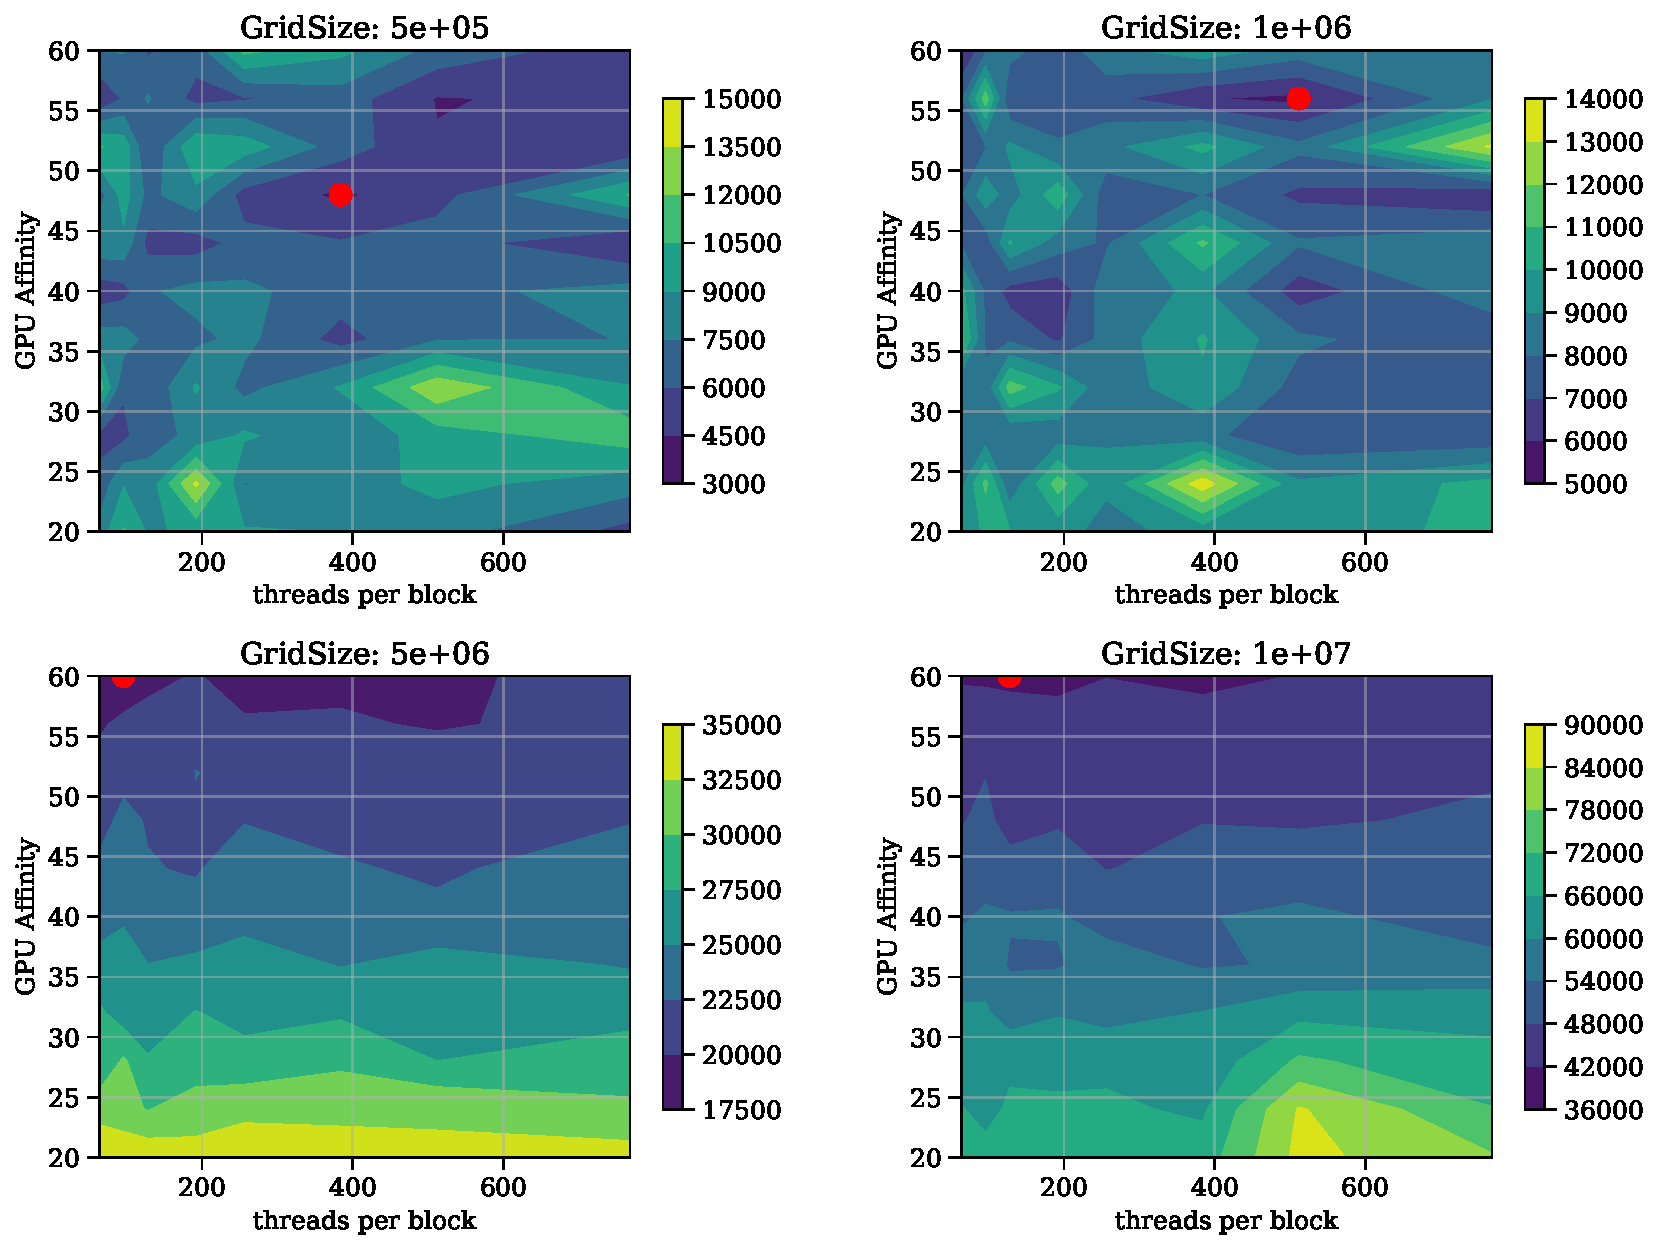
\includegraphics[width=\textwidth]{RawContourEulerClassictime}
        \caption{Classic decomposition}
        \label{f:EulerContourC}
    \end{subfigure}
    \begin{subfigure}[!tb]{.75\textwidth}
        \centering
        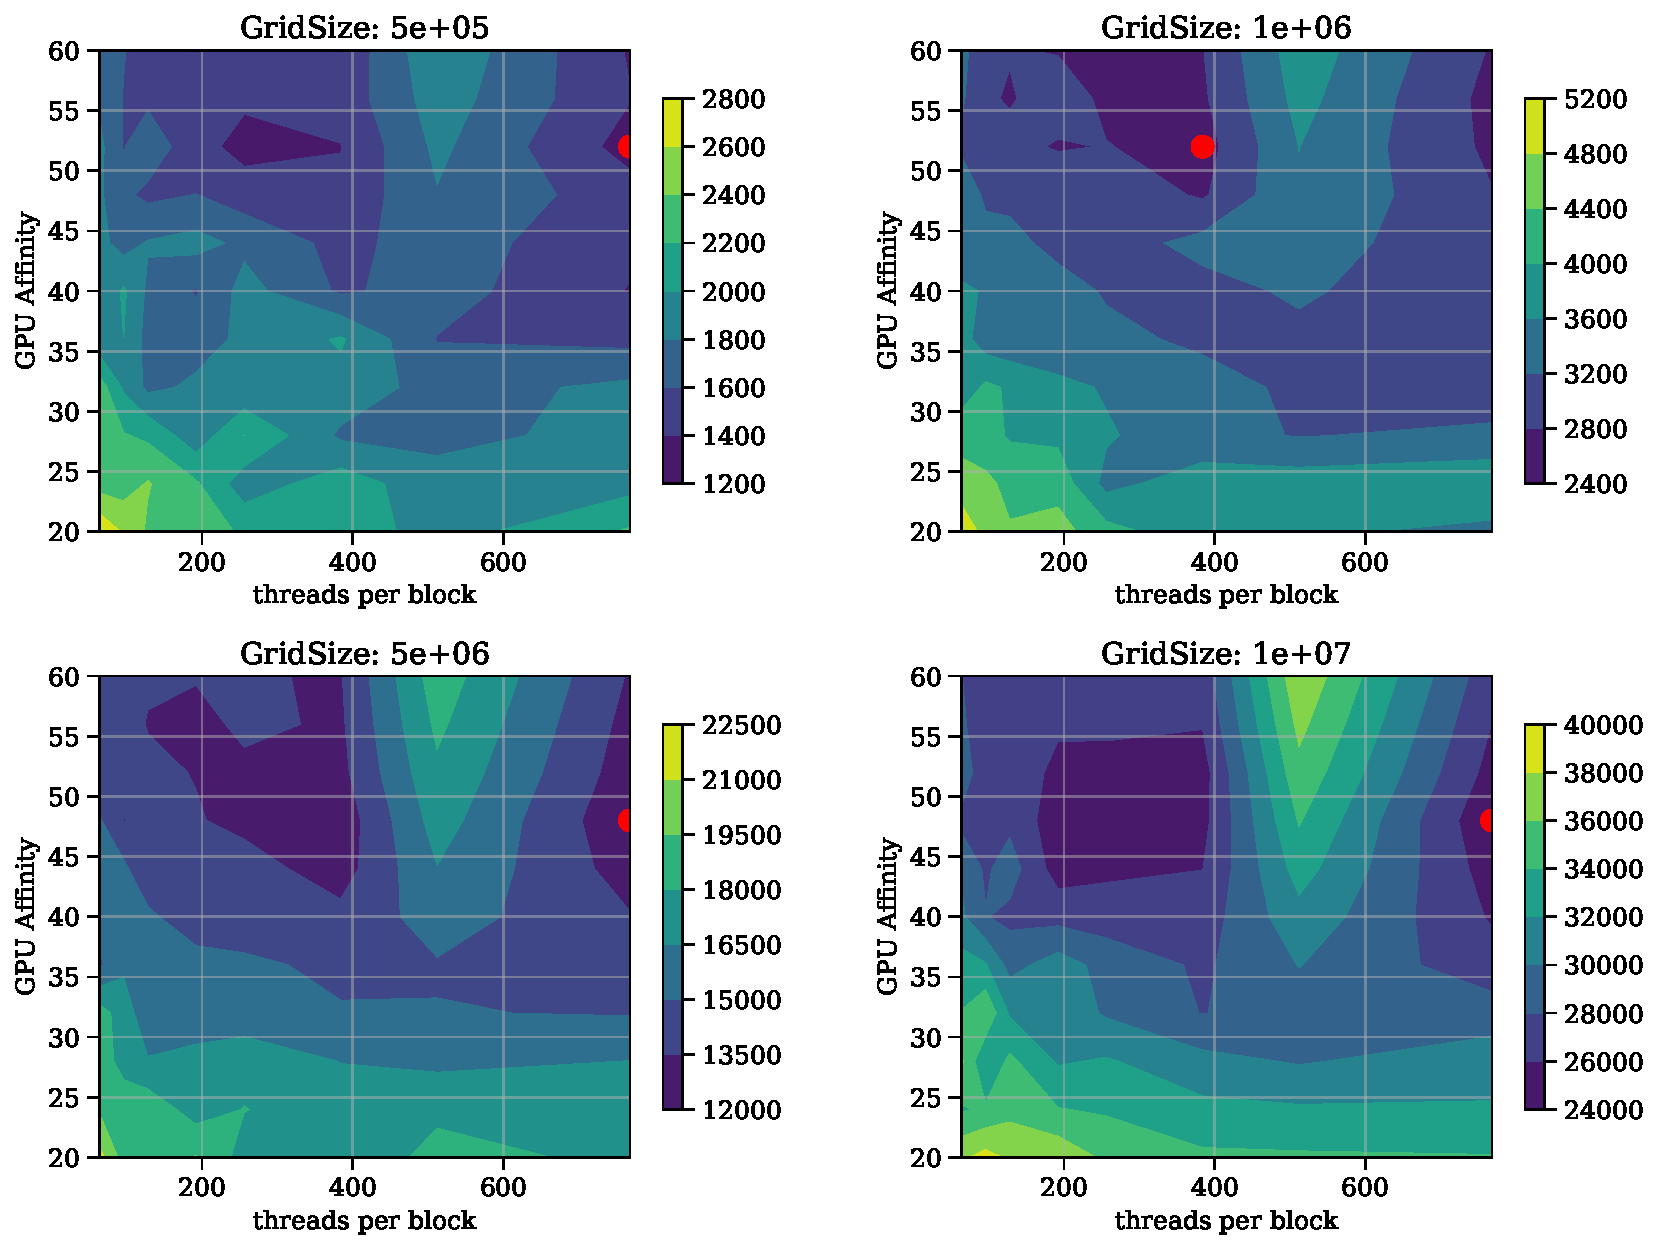
\includegraphics[width=\textwidth]{RawContourEulerSwepttime}
        \caption{Swept decomposition}
        \label{f:EulerContourS}
    \end{subfigure}
    \caption{A map of the time cost per timestep of the Euler equations at 4 grid sizes.
    The red dot signifies the best performance.}
    \label{f:EulerContours}
\end{figure}

\begin{figure}[htbp]
    \centering
    \begin{subfigure}[t]{.75\textwidth}
        \centering
        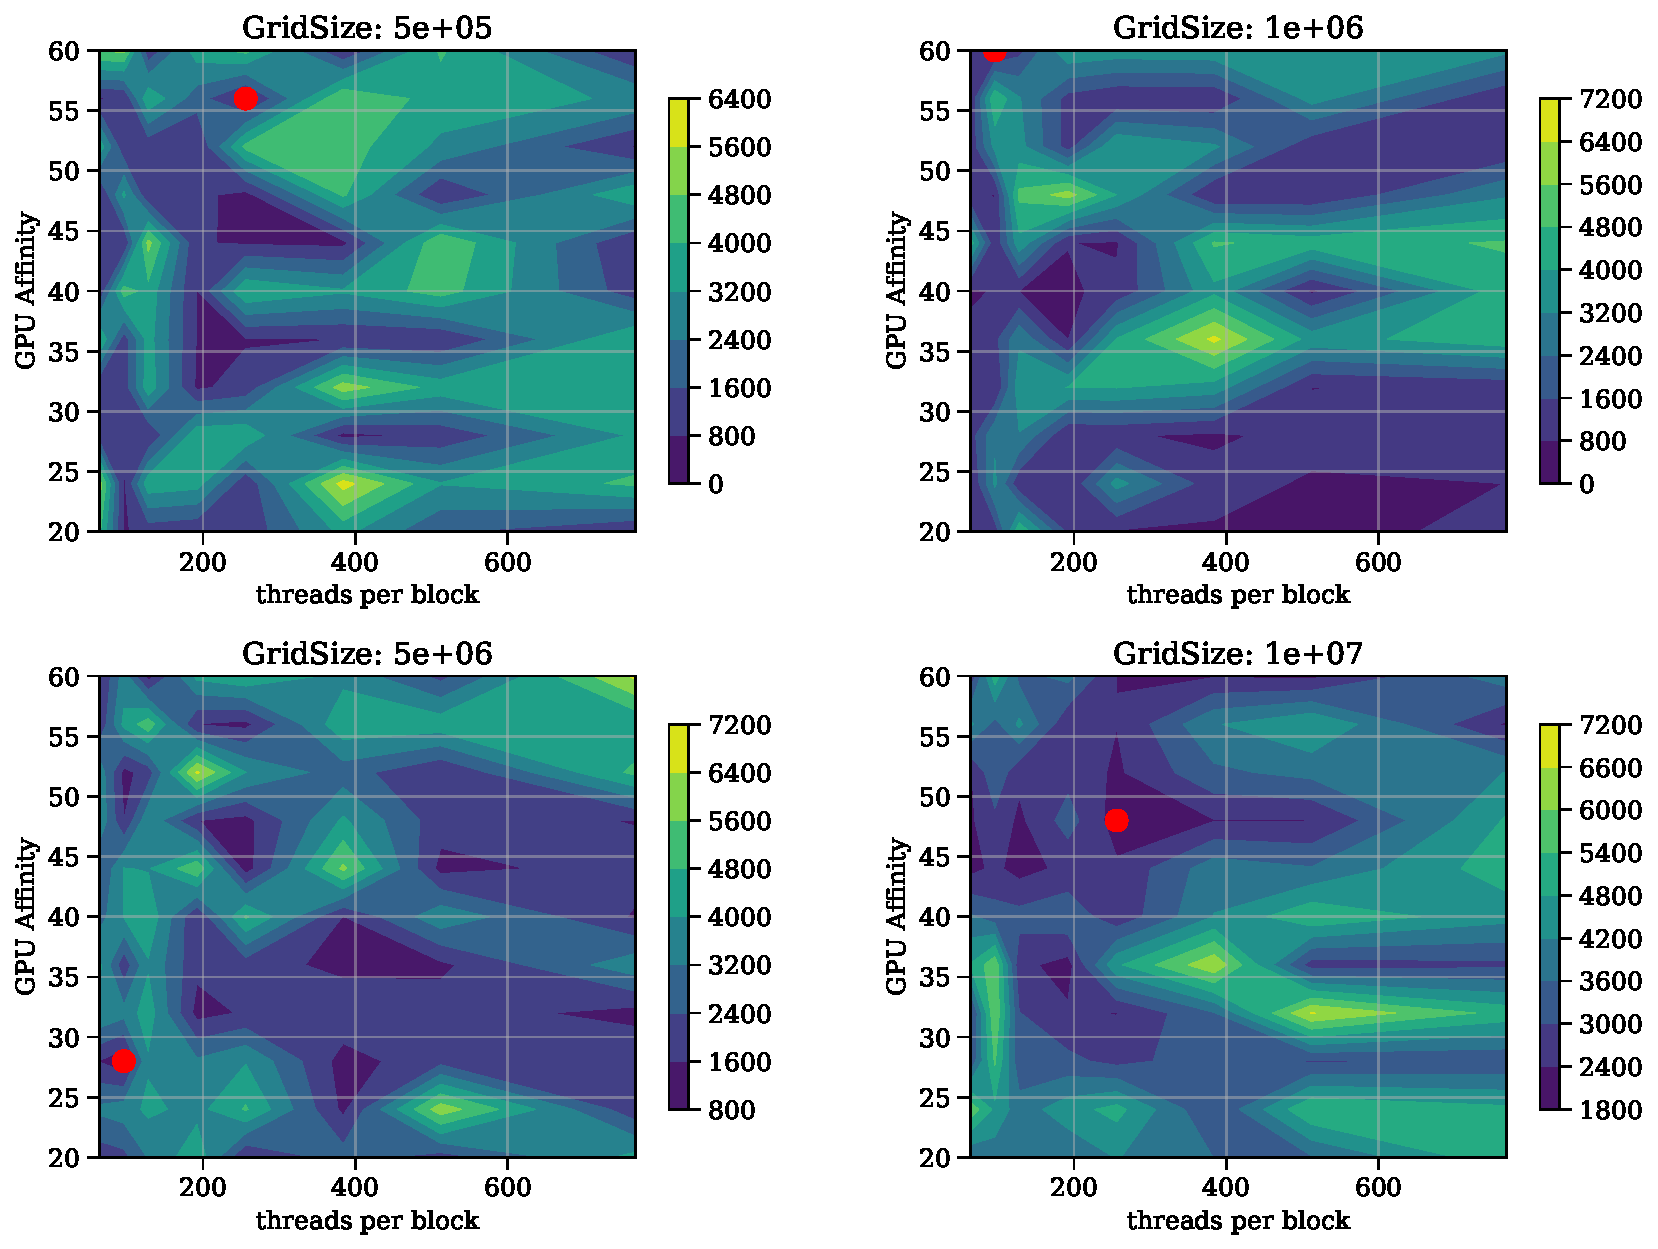
\includegraphics[width=\textwidth]{RawContourHeatClassictime}
        \caption{Classic decomposition}
        \label{f:HeatContourC}
    \end{subfigure}
    \begin{subfigure}[!tb]{.75\textwidth}
        \centering
        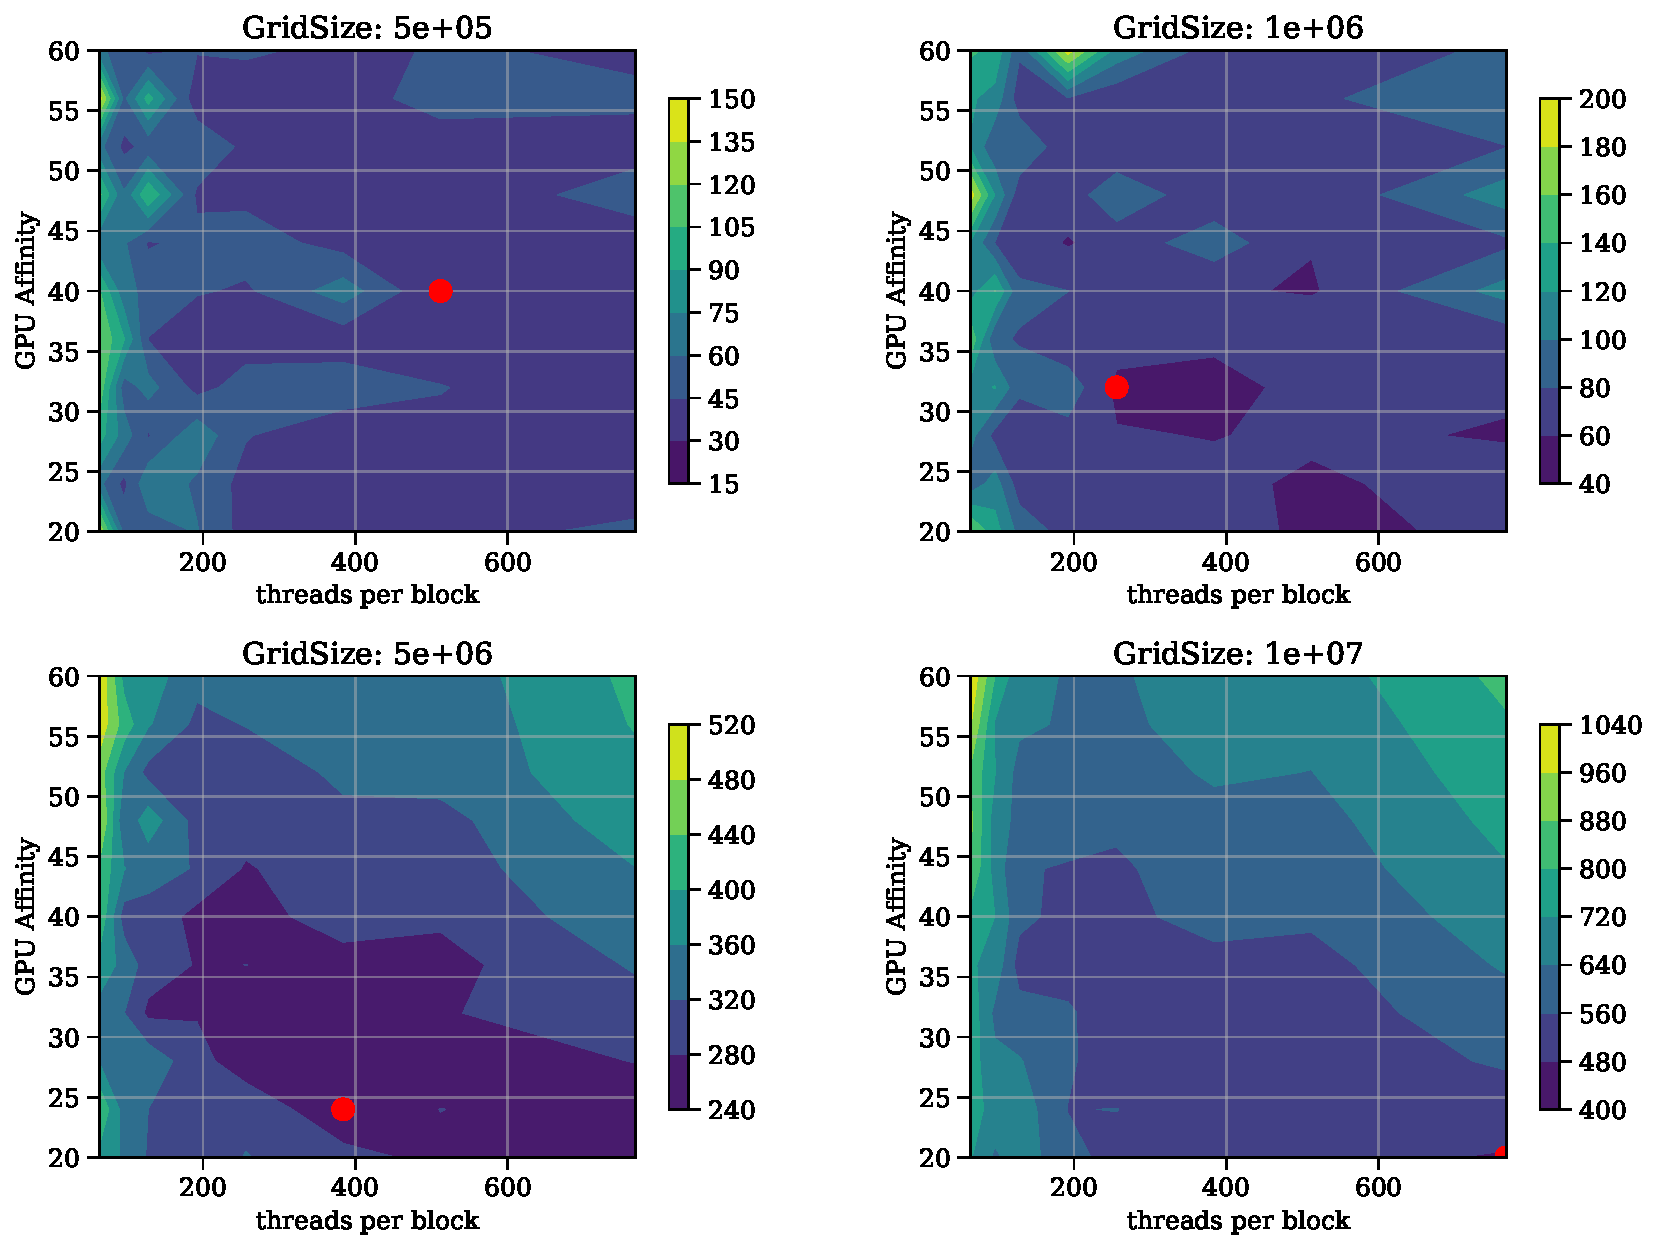
\includegraphics[width=\textwidth]{RawContourHeatSwepttime}
        \caption{Swept decomposition}
        \label{f:HeatContourS}
    \end{subfigure}
    \caption{A map of the time cost per time step of the heat equation at 4 grid sizes.
    The red dot signifies the best performance.}
    \label{f:HeatContours}
\end{figure}

Though we would emphasize that these results are representative of narrow experimental conditions,
architectures and design settings, the regularity of the \texttt{Swept} program performance
allows us to present fitted results in Table~\ref{tab:tablefit}, corresponding to the data points presented in Figures~\ref{f:BestRuntimeHeat} and ~\ref{f:BestRuntimeEuler}, that may illuminate and
guide future work on this and similar topics.

\begin{table}
\caption{Coefficients for power-law fit of grid size vs time per timestep ($y = Ax^b$) of \texttt{Swept} performance at best runtime configuration.}
%\vspace{-0.5em}
\label{tab:tablefit}
        \begin{center}
                \begin{tabular}{@{}l c c c}
                \toprule
                Equation & A & b & $R^2$ \\
                \midrule
                Euler   & \num{3.55e-3} & \num{0.976} & \num{0.999} \\
                Heat    & \num{1.08e-4} & \num{0.949} & \num{0.999} \\
                \bottomrule
                \end{tabular}
        \end{center}
\end{table}



\section{Conclusions} \label{sec:hConc}

We examined the performance characteristics of design choices that must be made when applying
the swept rule to partial differential equations on heterogeneous computational architectures using swept-time space decomposition.
These design choices are: how many threads per block---i.e., points per domain---to assign,
what proportion of the total domain to assign to a GPU, and how to efficiently and generally
store the working array throughout the simulation.

Our study aimed to answer the primary questions concerning these design choices laid out in Section~\ref{sec:obj1}.
First, we found that the best number of points to assign to each domain varies with the
algorithm, governing equation(s), and grid size.
To achieve the best performance on repeated similar runs, any program should be tested
over a limited number of time steps and tuned to the best result;
however, in general we recommend choosing a per-process domain size value from \SIrange{96}{384}
that is a multiple of \num{32}.
This is consistent with our previous results for the GPU-only implementation of the swept rule.
Next, we concluded that while a GPU affinity is best chosen after a similar tuning experiment,
for more complex equations an affinity from \SIrange{40}{60} performs well and an affinity
from \SIrange{20}{40} does best for simpler problems.
Next, there is a significant tradeoff between extensibility and performance associated with the primary data structure and compression scheme applied to the working quantity in the simulation.
We choose to continue working with the \texttt{lengthening} method despite its performance drawbacks
because it simplifies development substantially and has facilitated the development of this framework with which we can continue to develop codes and tests based on the swept rule.
Finally, although any conclusions drawn from an experiment on only two nodes are limited,
we showed a significant relative improvement over our previous results for the Euler equations
using a fine-tuned GPU-only program~\cite{OurJCP}.

Future work in this project will continue adapting the swept rule to higher dimensions, architecture types, and grid formations.
For example, while Alhubail and Wang demonstrated the two-dimensional swept rule for CPU-based clusters~\cite{Alhubail:2016arxiv}, we have not yet extended this to heterogeneous systems.
In addition, we recognize the need to develop new experiments that examine the scaling characteristics of the program as additional computational resources are added.
We plan on and executing those experiments on cloud systems like Amazon Web Services, Microsoft Azure, or Nvidia GPU Cloud. 
As we conduct these experiments, we hope to gain greater insight into the factors affecting performance and develop a more robust performance model for the swept rule.


\section*{Acknowledgments}

This material is based upon work supported by NASA under award No.~NNX15AU66A
under the technical monitoring of Drs.~Eric Nielsen and Mujeeb Malik.
We also gratefully acknowledge the support of Nvidia Corporation for donated
Tesla K40c GPU used for this research.

\section*{References}
\bibliographystyle{elsarticle-num}
\bibliography{paper-heterogeneous-swept}

\end{document}
